%!TEX root = ../root.tex
\section{Introduction}

The robustness of autonomous vehicles has increased prodigiously in the recent years. While long-range autonomous driving on the highway has been around for decades already~\cite{Pomerleau_1996_616}, advances in mapping, 3D data processing and computer vision have enabled cars to drive autonomously for thousands of miles in unconstrained, city environments~\cite{urmson2008autonomous}. While this surely is an impressive feat, one quickly notes that most of these miles have been logged in California weather, which provides optimal operating conditions for sensors such as LiDARs. In order for these systems to gain acceptance worldwide, it is crucial that they could be operated in more challenging weather conditions, such as rain, fog and snow. 

As we strive to make autonomous vehicles more adaptable to varying weather conditions, it is important to understand how sensors will behave in such conditions. Of particular interest, snowy conditions may cause challenging situations for sensors such as LiDARs. Indeed, the laser beams emitted may illuminate the snowflakes themselves, thus providing echoes that do not correspond to real obstacles. Consider fig.~\ref{fig:good-bad-weather} for example. The same scene appears drastically different depending on whether it was captured on a clear or snowy day. While programmable lighting may help circumvent this problem~\cite{tamburo2014programmable}, current LiDARs may fail under such circumstances. 

In this paper, our main contribution is to provide a characterization of the behavior of four well-known LiDARs in snowy conditions. Through an extensive empirical study performed on a novel dataset captured under varying degrees of snowfall, we evaluate how much these LiDARs are sensitive---or not---to falling snow. We show that recent advances in sensor design have increased their robustness even to significant snowfall. 

\begin{figure}
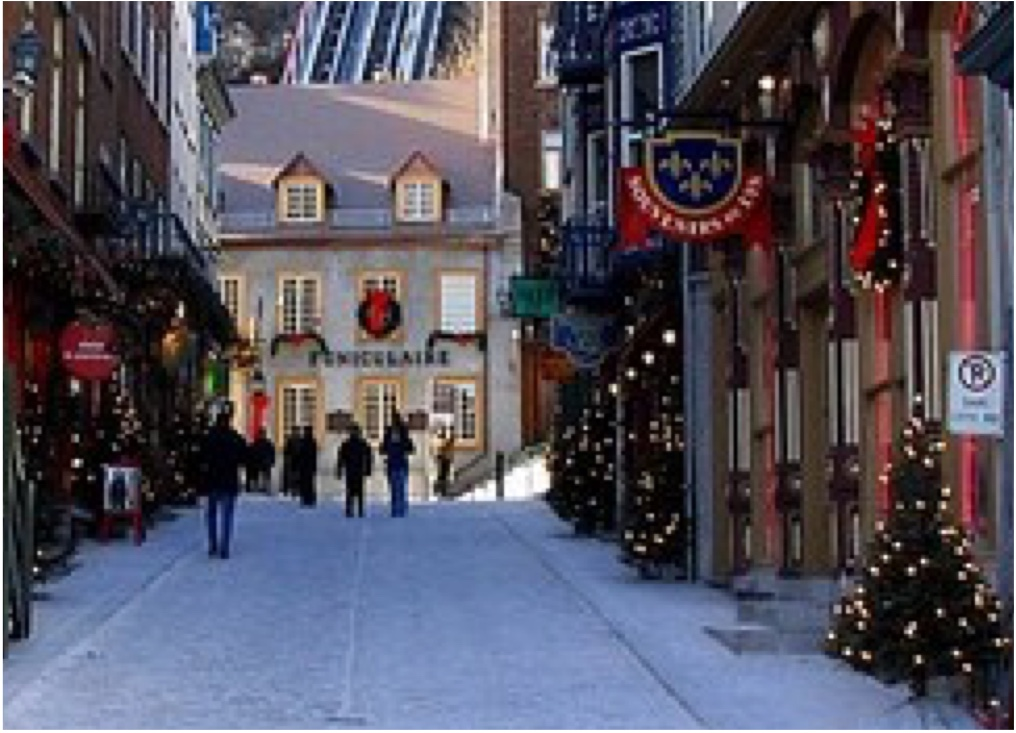
\includegraphics[width=.48\linewidth]{./img/teaser/summer.jpg}
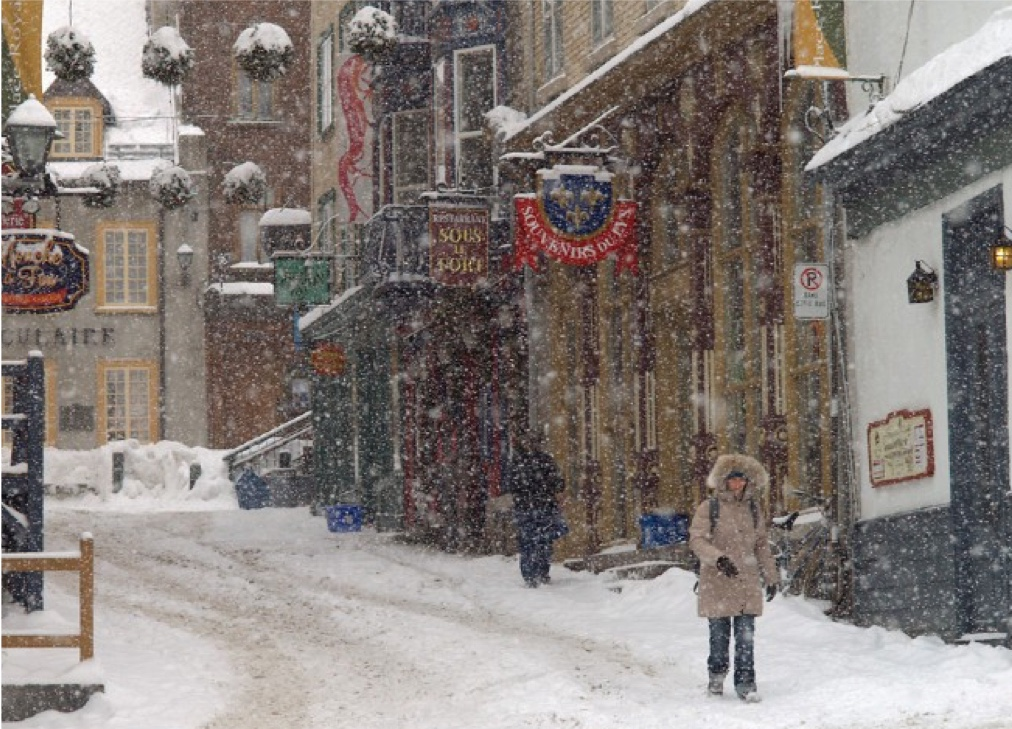
\includegraphics[width=.48\linewidth]{./img/teaser/winter.jpg}
\caption{Driving in bad weather. While autonomous vehicles have attained a great level of performance in nice weather (left), bad weather can cause significant challenges due to limited visibility (right). In this paper, we characterize the behavior in snowy conditions for oft-used sensors in autonomous cars: LiDARs. \emph{Photo credit}: Nicole Duchesne (left), Gaetan Chevalier (right).}
\label{fig:good-bad-weather}
\end{figure}

\subsection{Related work}

It is well-known that snow poses significant challenges to sensors mounted on-board outdoor mobile robots or other autonomous vehicles. For example, in their Antarctica exploration project, Moorehead et al. indicate that ``in heavy [snow] storms, [...] the laser could not be used''~\cite{Moorehead_1999_2122}. Similarly, Yamauchi et al. relate that ``LiDAR and stereo vision provide greater accuracy and resolution in clear weather but has difficulty with precipitation and obscurants''~\cite{yamauchi2010fusing}. Common approaches for dealing with this problem include filtering 3-D data~\cite{Moorehead_1999_2122}, or video~\cite{barnum2010analysis}, but this is often not enough to completely remove artifacts. 

It is therefore important to characterize how sensors behave in such conditions. To this end, Sumi et al.~\cite{sumi-arso-13} build a specifically-designed simulated-snow chamber, with white polystyrene beads flown with large fans to simulate snow. In our case, we use real-world conditions to acquire a novel dataset of more than 6 days of snowfall.

Finally, we also mention the work of Servomaa et al.~\cite{servomaa2002snowfall}, who use LiDARs (and other sensors) to characterize snow storms for monitoring and measurement applications. In our case, we characterize the behavior of the sensors themselves for robotics applications.

% Less related: ground-penetrating radar to analyze polar ice-sheets~\cite{lever2013autonomous}. 



% autonomous vehicles more and more robust (cite efforts from Google/CMU/etc.)
% thousands of miles accumulated
% but in what weather? 

% as we strive to make autonomous vehicles more adaptable to various weather conditions, it's important to understand how sensors behave in such conditions. 
% of particular interest, snowy conditions may cause challenging situations for ... 
% show example of particularly bad snow scenes
% vision in bad weather (Srinivas) -- active lighting
% characterization of _real_ sensors, in _real_ snowy conditions, ranging from ... to ... 

% through a thorough analysis of this novel dataset, we show that most of the 3D sensors are indeed robust to significant snowfall (due to their own internal filtering algorithms), and that they're ok to work ``out of the box''. 

